\documentclass[xcolor=pdflatex,dvipsnames,table]{beamer}
\usepackage{epsfig,graphicx}
\usepackage{palatino}
\usepackage{fancybox}
\usepackage{relsize}
\usepackage[procnames]{listings}
\usepackage{hyperref}
\usepackage{qtree} % needed?
\usepackage{booktabs}
\usepackage{dirtree}
\usepackage[normalem]{ulem}


% fatter TT font
\renewcommand*\ttdefault{txtt}
% another TT, suggested by Alex
% \usepackage{inconsolata}
% \usepackage[T1]{fontenc} % needed as well?


\newcommand{\scale}{0.7}

\newcommand{\todo}[1]{{\emph{TODO: #1}}}
\newcommand{\martin}[1]{{\color{blue} Martin: #1}}
\newcommand{\abcdef}[1]{{\color{red} Author2: #1}}

% uncomment following for final submission
%\renewcommand{\todo}[1]{}
%\renewcommand{\martin}[1]{}
%\renewcommand{\author2}[1]{}

\newcommand{\code}[1]{{\texttt{#1}}}

\hypersetup{
  linkcolor  = black,
%  citecolor  = blue,
  urlcolor   = blue,
  colorlinks = true,
}

\beamertemplatenavigationsymbolsempty
\setbeamertemplate{footline}[frame number]





\newif\ifbook
% shared in slides and book

\lstdefinelanguage{chisel}{
%  morekeywords={abstract,case,catch,class,def,%
%    do,else,extends,false,final,finally,%
%    for,if,implicit,import,match,mixin,%
%    new,null,object,override,package,%
%    private,protected,requires,return,sealed,%
%    super,this,throw,trait,true,try,%
%    type,val,var,while,with,yield},
%  otherkeywords={=>,<-,<\%,<:,>:,\#,@},
  sensitive=true,
  morecomment=[l]{//},
  morecomment=[n]{/*}{*/},
  morestring=[b]",
  morestring=[b]',
  morestring=[b]"""
}

\usepackage{color}
\definecolor{dkgreen}{rgb}{0,0.6,0}
\definecolor{gray}{rgb}{0.5,0.5,0.5}
\definecolor{mauve}{rgb}{0.58,0,0.82}

% Default settings for code listings
%\ifbook
\lstset{%frame=lines,
  language=chisel,
  aboveskip=3mm,
  belowskip=3mm,
  showstringspaces=false,
  columns=fixed, % basewidth=\mybasewidth,
  basicstyle={\small\ttfamily},
  numbers=none,
  numberstyle=\footnotesize,
  % identifierstyle=\color{red},
  breaklines=true,
  breakatwhitespace=true,
  procnamekeys={def, val, var, class, trait, object, extends},
  % procnamestyle=\ttfamily,
  tabsize=2,
  float
}
%\else
%\lstset{%frame=lines,
%  language=chisel,
%  aboveskip=3mm,
%  belowskip=3mm,
%  showstringspaces=false,
%  columns=fixed, % basewidth=\mybasewidth,
%  basicstyle={\small\ttfamily},
%  numbers=none,
%  numberstyle=\footnotesize\color{gray},
%  % identifierstyle=\color{red},
%  keywordstyle=\color{blue},
%  commentstyle=\color{dkgreen},
%  stringstyle=\color{mauve},
%  breaklines=true,
%  breakatwhitespace=true,
%  procnamekeys={def, val, var, class, trait, object, extends},
%  procnamestyle=\ttfamily\color{red},
%  tabsize=2,
%  float
%}
%\fi

\lstnewenvironment{chisel}[1][]
{\lstset{language=chisel,#1}}
{}

\newcommand{\shortlist}[1]{{\lstinputlisting[nolol]{#1}}}

\newcommand{\longlist}[3]{{\lstinputlisting[float, caption={#2}, label={#3}, frame=tb, captionpos=b]{#1}}}

\newcommand{\verylonglist}[3]{{\lstinputlisting[caption={#2}, label={#3}, frame=tb, captionpos=b]{#1}}}


\title{Finite-State Machines}
\author{Martin Schoeberl}
\date{\today}
\institute{Technical University of Denmark\\
Embedded Systems Engineering}

\begin{document}

\begin{frame}
\titlepage
\end{frame}

\begin{frame}[fragile]{Overview}
\begin{itemize}
\item Debugging with waveforms
\item Fun with counters
\item Finite-state machines
\item Collection with \code{Vec}
\end{itemize}
\end{frame}

\begin{frame}[fragile]{Lab Work}
\begin{itemize}
\item Looks like it went fine last week
\item This week it will be counters to test the 7-segment display
\item Got a question: ``Due to the corona out-break, what will happen to our vending machine project if DTU closes down? Will the project get cancelled? or will we all fail the course, because personally I cannot work on the project without any help from the TAs.''
\item DTU has closed down from today on
\item No one should fail because of the Corona outbreak!
\item We will find a flexible solution for the lab work
\begin{itemize}
\item I really want you to get hands on experience to design stuff!
\end{itemize}
\item I do not want that your grade is based only on the written exam
\end{itemize}
\end{frame}

\begin{frame}[fragile]{Testing with Chisel}
\begin{itemize}
\item Set input values with \code{poke}
\item Advance the simulation with \code{step}
\item Read the output values with \code{peek}
\item Compare the values with \code{expect}
\item Import following packages:
\shortlist{../code/test_import.txt}
\end{itemize}
\end{frame}

\begin{frame}[fragile]{Using \code{peek}, \code{poke}, and \code{expect}}
\begin{chisel}
// Set input values
poke(dut.io.a, 3)
poke(dut.io.b, 4)
// Execute one iteration
step(1)
// Print the result
val res = peek(dut.io.result)
println(res)

// Or compare against expected value
expect(dut.io.result, 7)
\end{chisel}
\end{frame}

\begin{frame}[fragile]{A Chisel Tester}
\begin{itemize}
\item Extends class \code{PeekPokeTester}
\item Has the device-under test (DUT) as parameter
\item Testing code can use all features of Scala
\end{itemize}
\begin{chisel}
class CounterTester(dut: Counter) extends PeekPokeTester(dut) {

  // Here comes the Chisel/Scala code
  // for the testing
}
\end{chisel}
\end{frame}

\begin{frame}[fragile]{Using ScalaTest for our Tester}
\begin{itemize}
\item Little verbose syntax
\item Copy example code to start with
\end{itemize}
\shortlist{../code/scalatest_simple.txt}
\end{frame}

\begin{frame}[fragile]{Generating Waveforms}
\begin{itemize}
\item Waveforms are timing diagrams
\item Good to see many parallel signals and registers
\item Additional parameters: \code{"--generate-vcd-output", "on"}
\item IO signals and registers are dumped
\item Generates a .vcd file
\item Viewing with GTKWave or ModelSim
\end{itemize}
\end{frame}

\begin{frame}[fragile]{A Self-Running Circuit}
\begin{itemize}
\item \code{SevenSegTest} is a self-running circuit
\item Needs no stimuli (\code{poke})
\item Just run for a few cycles
\item Tester for today's lab
\item This tester does NOT test the circuit
\begin{itemize}
\item You are not finished when this test does not show an error
\end{itemize}
\end{itemize}
\begin{chisel}
class SevenSegTest(dut: CountSevenSeg) extends PeekPokeTester(dut) {
  step(100)
}
\end{chisel}
\end{frame}

\begin{frame}[fragile]{Display Waveform with GTKWave}
\begin{itemize}
\item Run the tester: \code{sbt test}
\item Locate the .vcd file in test\_run\_dir/SevenSegCountSpecnnn
\item Start GTKWave
\item Open the .vcd file with
\begin{itemize}
\item File -- Open New Tab
\end{itemize}
\item Select the circuit
\item Drag and drop the interesting signals
\end{itemize}
\end{frame}



\begin{frame}[fragile]{Call the Tester for Waveform Generation}
\begin{itemize}
\item Using here ScalaTest
\item Note \code{Driver.execute}
\item Note \code{Array("--generate-vcd-output", "on")}
\end{itemize}
\begin{chisel}
class SevenSegCountSpec extends
  FlatSpec with Matchers {
  "SevenSegTest " should "pass" in {
  chisel3.iotesters.Driver
  .execute(Array("--generate-vcd-output", "on"),
    () => new CountSevenSeg)
    { c => new SevenSegTest(c)} should be (true) }
}
\end{chisel}
\end{frame}




\begin{frame}[fragile]{Counters as Building Blocks}
\begin{itemize}
\item Counters are versatile tools
\item Count events
\item Generate timing ticks
\item Generate a one-shot timer
\end{itemize}
\end{frame}

\begin{frame}[fragile]{Counting Up and Down}
\begin{itemize}
\item Up:
\shortlist{../code/when_counter.txt}
\item Down:
\shortlist{../code/down_counter.txt}
\end{itemize}
\end{frame}

\begin{frame}[fragile]{Generating Timing with Counters}
\begin{itemize}
\item Generate a \code{tick} at a lower frequency
\item We used it in Lab 1 for the blinking LED
\item Use it for today's lab
\item Use it for driving the display multiplexing at 1~kHz
\end{itemize}
\begin{figure}
  \includegraphics[scale=0.8]{../figures/tick_wave}
\end{figure}
\end{frame}


\begin{frame}[fragile]{The Tick Generation}
\shortlist{../code/sequ_tick_gen.txt}
\end{frame}

\begin{frame}[fragile]{Using the Tick}
\begin{itemize}
\item A counter running at a \emph{slower frequency}
\item By using the \code{tick} as an enable signal
\end{itemize}
\shortlist{../code/sequ_tick_counter.txt}
\end{frame}

\begin{frame}[fragile]{The \emph{Slow} Counter}
\begin{itemize}
\item Incremented every \code{tick}
\end{itemize}
\begin{figure}
  \includegraphics[scale=0.8]{../figures/tick_count_wave}
\end{figure}
\end{frame}

\begin{frame}[fragile]{A Timer}
\begin{itemize}
\item Like a kitchen timer
\item Start by loading a timeout value
\item Count down till 0
\item Assert \code{done} when finished
\end{itemize}
\end{frame}

\begin{frame}[fragile]{One-Shot Timer}
\begin{figure}
  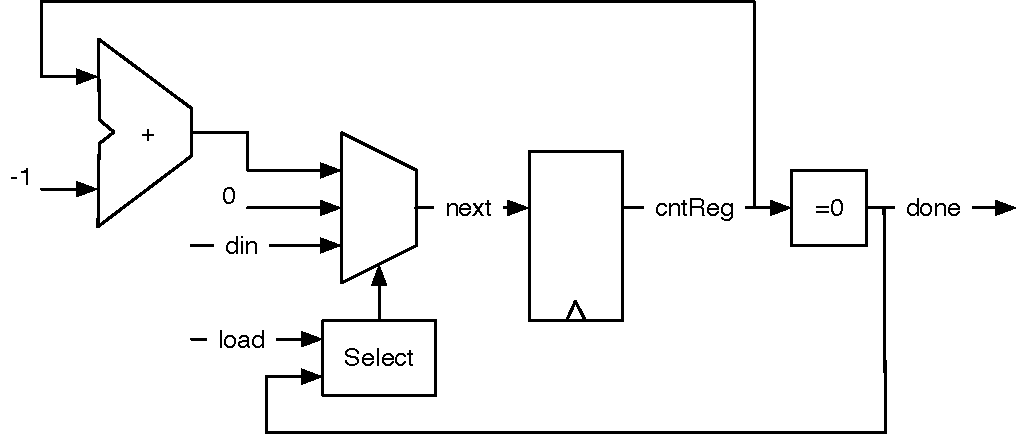
\includegraphics[scale=\scale]{../figures/timer}
\end{figure}
\end{frame}

\begin{frame}[fragile]{One-Shot Timer}
\shortlist{../code/timer.txt}
\end{frame}

\begin{frame}[fragile]{A 4 Stage Shift Register}
\begin{figure}
  \includegraphics[scale=\scale]{../figures/shiftregister}
\end{figure}
\shortlist{../code/shift_register.txt}
\end{frame}


\begin{frame}[fragile]{A Shift Register with Parallel Output}
\begin{figure}
  \includegraphics[scale=\scale]{../figures/shiftreg-paraout}
\end{figure}
\shortlist{../code/shift_paraout.txt}
\end{frame}

\begin{frame}[fragile]{A Shift Register with Parallel Load}
\begin{figure}
  \includegraphics[scale=0.5]{../figures/shiftreg-paraload}
\end{figure}
\shortlist{../code/shift_paraload.txt}
\end{frame}

\begin{frame}[fragile]{Midterm Evaluation}
\begin{itemize}
\item TODO: create a new form, no need for the graphics, as we are not live
\item An anonymous Google form (no login required)
\item 20 minutes time, including the break
\item We will look into it after the break
\end{itemize}
\begin{figure}
  \includegraphics[scale=0.5]{forms2020}
\end{figure}
\begin{itemize}
\item \url{https://forms.gle/wtvDrA4peD4oLvt16}
\end{itemize}
\end{frame}

\begin{frame}[fragile]{A Simple Circuit}
\begin{itemize}
\item What does the following circuit?
\item Is this related to a finite-state machine?
\end{itemize}
\begin{figure}
  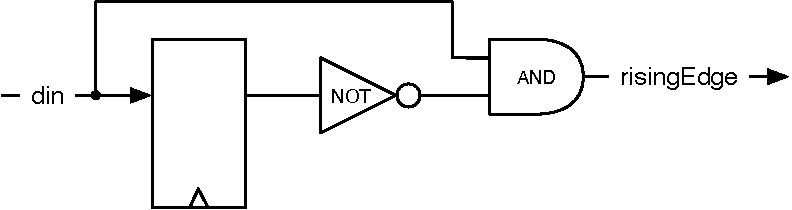
\includegraphics[scale=\scale]{../figures/fsm-rising}
\end{figure}
\end{frame}

\begin{frame}[fragile]{Finite-State Machine (FSM)}
\begin{itemize}
\item Has a register that contains the state
\item Has a function to computer the next state
\begin{itemize}
\item Depending on current state and input
\end{itemize}
\item Has an output depending on the state
\begin{itemize}
\item And maybe on the input as well
\end{itemize}
\item Every synchronous circuit can be considered a finite state machine
\item However, sometimes the state space is a little bit too large
\end{itemize}
\end{frame}

\begin{frame}[fragile]{Basic Finite-State Machine}
\begin{itemize}
\item A state register
\item Two combinational blocks
\end{itemize}
\begin{figure}
  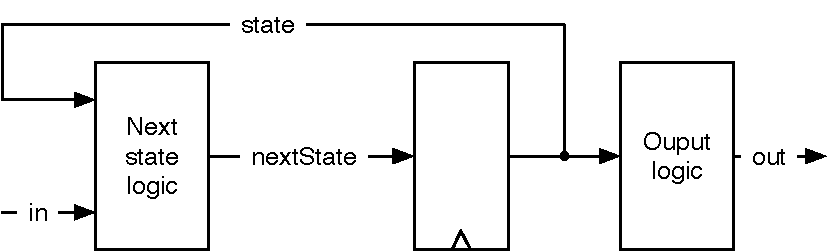
\includegraphics[scale=\scale]{../figures/fsm}
\end{figure}
\end{frame}

\begin{frame}[fragile]{State Diagram}
\begin{figure}
  \includegraphics[scale=\scale]{../figures/state-diag-moore}
\end{figure}
\begin{itemize}
\item States and transitions depending on input values
\item Example is a simple alarm FSM
\item Nice visualization
\item Will not work for large FSMs
\item Complete code in the Chisel book
\end{itemize}
\end{frame}


\begin{frame}[fragile]{State Table for the Alarm FSM}
\begin{table}
\centering
\begin{tabular}{ccccc}
\toprule
& \multicolumn{2}{c}{Input} \\
\cmidrule{2-3}
State &  Bad event & Clear & Next state & Ring bell \\
\midrule
green & 0 & 0 & green & 0 \\
green & 1 & - & orange & 0 \\
orange & 0 & 0 & orange & 0 \\
orange & 1 & - & red & 0 \\
orange & 0 & 1 & green & 0 \\
red & 0 & 0 & red & 1 \\
red & 0 & 1 & green & 1 \\
\bottomrule
\end{tabular}
\label{tab:state:table}
\end{table}
\end{frame}

\begin{frame}[fragile]{The Input and Output of the Alarm FSM}
\begin{itemize}
\item Two inputs and one output
\end{itemize}
\shortlist{../code/simple_fsm_io.txt}
\end{frame}

\begin{frame}[fragile]{Encoding the State}
\begin{itemize}
\item We can optimize state encoding
\item Two common encodings are: binary and one-hot
\item We leave it to the synthesize tool
\item Use symbolic names with an \code{Enum}
\item Note the number of states in the \code{Enum} construct
\item We use a Scala list with the \code{::} operator
\end{itemize}
\shortlist{../code/simple_fsm_states.txt}
\end{frame}

\begin{frame}[fragile]{Start the FSM}
\begin{itemize}
\item We have a starting state on reset
\end{itemize}
\shortlist{../code/simple_fsm_register.txt}
\end{frame}


\begin{frame}[fragile]{The Next State Logic}
\shortlist{../code/simple_fsm_next.txt}
\end{frame}

\begin{frame}[fragile]{The Output Logic}
\shortlist{../code/simple_fsm_output.txt}
\end{frame}

\begin{frame}[fragile]{Summary on the Alarm Example}
\begin{itemize}
\item Three elements:
\begin{enumerate}
\item State register
\item Next state logic
\item Output logic
\end{enumerate}
\item This was a so-called Moore FSM
\item There is also a FSM type called Mealy machine
\end{itemize}
\end{frame}

\begin{frame}[fragile]{A so-called Mealy FSM}
\begin{itemize}
\item Similar to the former FSM
\item Output also depends in the input
\item It is \emph{faster}
\item Less composable (draw it)
\end{itemize}
\begin{figure}
  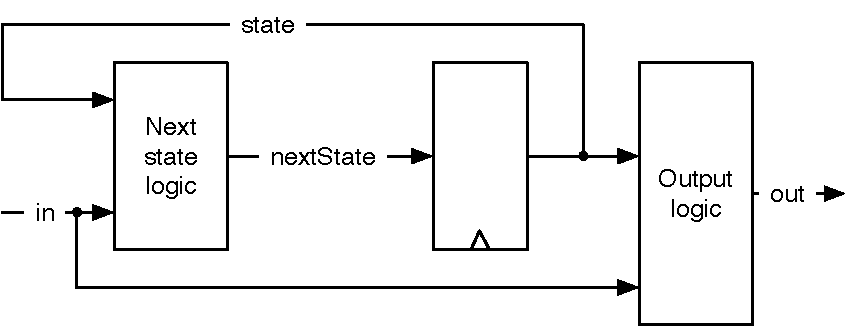
\includegraphics[scale=\scale]{../figures/mealy}
\end{figure}
\end{frame}

\begin{frame}[fragile]{The Mealy FSM for the Rising Edge}
\begin{itemize}
\item That was our starting example
\item Output is also part of the transition arrows
\end{itemize}
\begin{figure}
  \includegraphics[scale=\scale]{../figures/state-diag-mealy}
\end{figure}
\end{frame}

\begin{frame}[fragile]{The Mealy Solution}
\begin{itemize}
\item Show code from the book as it is too long for slides
\end{itemize}
\end{frame}

\begin{frame}[fragile]{State Diagram for the Moore Rising Edge Detection}
\begin{itemize}
\item We need three states
\end{itemize}
\begin{figure}
  \includegraphics[scale=\scale]{../figures/state-diag-rising-moore}
\end{figure}
\end{frame}

\begin{frame}[fragile]{Comparing with a Timing Diagram}
\begin{itemize}
\item Moore is delayed one clock cycle compared to Mealy
\end{itemize}
\begin{figure}
  \includegraphics[scale=1]{../figures/rising}
\end{figure}
\end{frame}

\begin{frame}[fragile]{What is Better?}
\begin{itemize}
\item It depends ;-)
\item Moore is on the save side
\item More is composable
\item Mealy has \emph{faster} reaction
\item Both are tools in you toolbox
\item Keep it simple with your vending machine and use a Moore FSM
\end{itemize}
\end{frame}

\begin{frame}[fragile]{Another Simple FSM}
\begin{itemize}
\item a FSM for a single word buffer
\item Just two symbols for the state machine
\end{itemize}
\begin{chisel}
  val empty :: full :: Nil = Enum(2)
\end{chisel}
\end{frame}

\begin{frame}[fragile]{Finite State Machine for a Buffer}
\begin{chisel}
  val empty :: full :: Nil = Enum(2)
  val stateReg = RegInit(empty)
  val dataReg = RegInit(0.U(size.W))

  when(stateReg === empty) {
    when(io.enq.write) {
      stateReg := full
      dataReg := io.enq.din
    }
  }.elsewhen(stateReg === full) {
    when(io.deq.read) {
      stateReg := empty
    }
  }
\end{chisel}
\begin{itemize}
\item A simple buffer for a bubble FIFO
\end{itemize}
\end{frame}

\begin{frame}[fragile]{A Collection of Signals with \code{Vec}}
\begin{itemize}
\item Chisel \code{Vec} is a collection of signals of the same type
\item The collection can be accessed by an index
\item Similar to an array in other languages
\item Wrap into a \code{Wire()} for combinational logic
\item Wrap into a \code{Reg()} for a collection of registers
\end{itemize}
\shortlist{../code/vec.txt}
\end{frame}

\begin{frame}[fragile]{Using a \code{Vec}}
\shortlist{../code/vec_access.txt}
\begin{itemize}
\item Reading from an \code{Vec} is a multplexer
\item We can put a \code{Vec} into a \code{Reg}
\end{itemize}
\shortlist{../code/reg_file.txt}
\noindent An element of that register file is accessed with an index and used as a normal register.

\shortlist{../code/reg_file_access.txt}
\end{frame}


\begin{frame}[fragile]{Mixing Vecs and Bundles}
\begin{itemize}
\item We can freely mix bundles and vectors
\item When creating a vector with a bundle
type, we need to pass a prototype for the vector fields. Using our
\code{Channel}, which we defined above, we can create a vector of channels with:
\end{itemize}
\shortlist{../code/vec_bundle.txt}
\begin{itemize}
\item A bundle may as well contain a vector
\end{itemize}
\shortlist{../code/bundle_vec.txt}
\end{frame}

\begin{frame}[fragile]{Today's Lab}
\begin{itemize}
\item Driving your 7-segment decoder
\item Use a counter to count from 0 to 15, driving your display
\item Use another counter to generate your timing
\begin{itemize}
\item We talked about this today
\end{itemize}
\item You clock on the board is 100 MHz
\item The given tester does only generate a waveform, no testing
\item Use a different maximum count value for waveform debugging
\item Then synthesize it for the FPGA
\item (Show a TA your working design)
\item \href{https://github.com/schoeberl/chisel-lab/tree/master/lab6}{Lab 6}
\end{itemize}
\end{frame}

\begin{frame}[fragile]{Summary}
\begin{itemize}
\item Waveform testing is the way to develop/debug
\item Counters are important tools, e.g., to generate timing
\item Finite-state machines are another tool of the trade
\item Two types: Moore and Mealy
\item A Chisel \code{Vec} is the hardware version of an array
\end{itemize}
\end{frame}


\end{document}

%\begin{frame}[fragile]{xxx}
%\begin{itemize}
%\item yyy
%\end{itemize}
%\end{frame}
